\section{目的與規格對照}
依 Lab 7（PDF 第 26--30 頁）完成三項模擬：固定基體偏壓比較 N=3、5、7 的環形振盪器；固定級數比較四種基體接法；掃描 NMOS 與 PMOS 的反向 source-body 偏壓並觀察臨界電壓。兩個 netlist 共五個變體全部完成，環形振盪器在同一變體內同時包含三種級數。

\section{電路與理論}
每級反相器使用 $W_n=0.6\,\mu$m、$W_p=1.8\,\mu$m、$L=0.25\,\mu$m。最後一級回接第一級，形成奇數級反相回授；沒有外接振盪時脈。為打破完全對稱的數值初始狀態，以 UIC 與一個節點 0.05 V 的初始條件啟動，這是暫態啟動方法，並非物理上無擾動啟振能力的驗證。

若每級平均延遲為 $t_p$，則 $T\approx2Nt_p$、$f\approx1/(2Nt_p)$。四種 body 設定依序為：PMOS body=1 V、NMOS body=0 V；只把 PMOS body 提高至 1.2 V；只把 NMOS body 降為 -0.2 V；兩者皆改。講義在 2.5 V 電源使用的 0.5 V 偏移，本次按相同比例調為 0.2 V。

NMOS 的長通道 body-effect 關係為
\[V_{tn}=V_{tn0}+\gamma\left(\sqrt{2\phi_F+V_{SB}}-\sqrt{2\phi_F}\right).\]
PMOS 使用相應的反向偏壓與臨界電壓絕對值。模型中的短通道、汲極偏壓及其他效應仍由模擬器處理，沒有自行指定不可取得的 $\gamma$ 或 $\phi_F$。

\section{模擬設定與量測定義}
本次使用獨立提供的 MOS 模型，電源為 1.0 V、溫度為 $27\,^{\circ}$C，並保留講義的電路拓樸及下列比較條件。1 V 是本次模擬設定，並非由公開模型文件確認的元件額定值；不能把講義舊製程的數值當成此次模型的驗收值。

模擬使用 HSPICE S-2021.09、RUNLVL=6。表格取自實際原生量測結果，圖形由實際列印數據重繪；每個變體都完整重設掃描參數及溫度，避免前一個變體的設定殘留。數值求解完成與量測成功，不等於已驗證製程可靠度。加密模型區塊的內部警告仍無法完整檢視。
環形振盪器模擬 20 ns，列印步距 1 ps；跳過前 10 ns，在 50\% 門檻的第 1 與第 6 個上升交越間量測五個週期，再以 $f=5/\Delta t$ 求平均頻率。另對 source 電壓作 0--1 V、10 mV 步距的 DC 掃描，直接列印 VTH，而非由任意電流門檻推估。

\section{實測結果}
下表單位 GHz；所有頻率均來自啟動後的實際交越時間。

\begin{center}\small
\begin{tabular}{llll}
\toprule
偏壓配置 & N=3 & N=5 & N=7 \\
\midrule
基準 & 2.0095 & 1.1609 & 0.8279 \\
僅 PMOS 反偏 & 1.9266 & 1.1101 & 0.7916 \\
僅 NMOS 反偏 & 1.8870 & 1.0955 & 0.7814 \\
雙側反偏 & 1.8112 & 1.0493 & 0.7485 \\
\bottomrule
\end{tabular}
\end{center}
\begin{figure}[htbp]
\centering
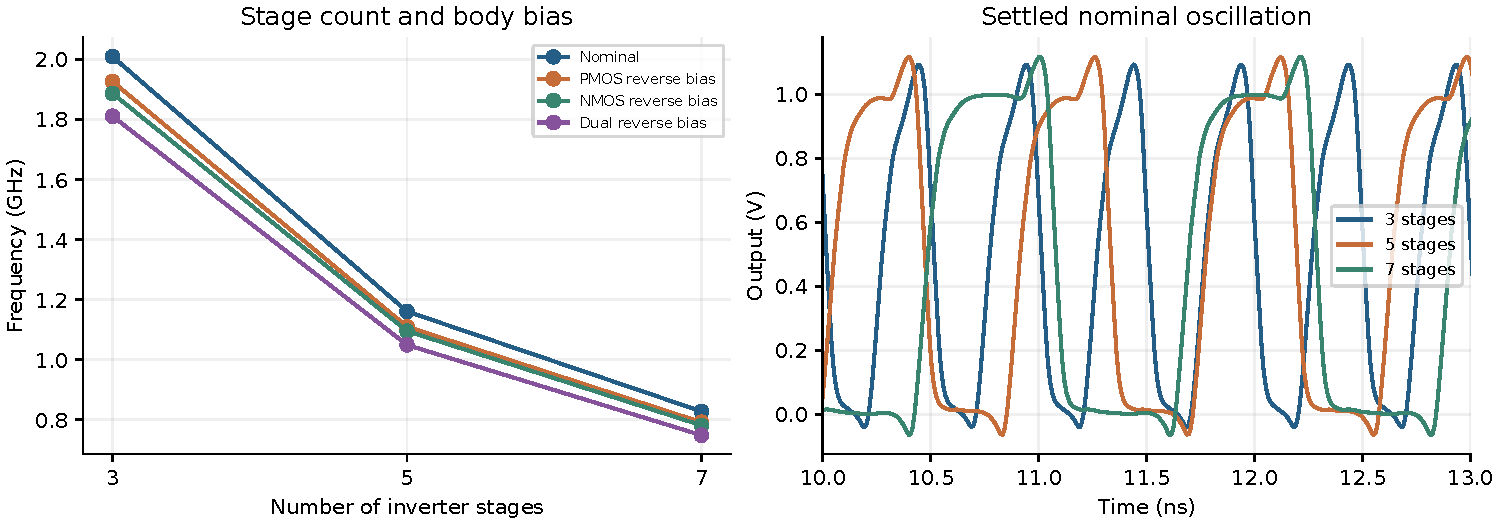
\includegraphics[width=\linewidth]{figures/ring_body_bias.pdf}
\caption{級數、基體反向偏壓與振盪頻率，以及基準波形。}
\end{figure}
\begin{center}\small
\begin{tabular}{llll}
\toprule
元件 & Bias=0 V & Bias=1 V & Change (mV) \\
\midrule
NMOS & 0.3951 & 0.5804 & 185.29 \\
PMOS magnitude & 0.3364 & 0.5028 & 166.43 \\
\bottomrule
\end{tabular}
\end{center}
\begin{figure}[htbp]
\centering
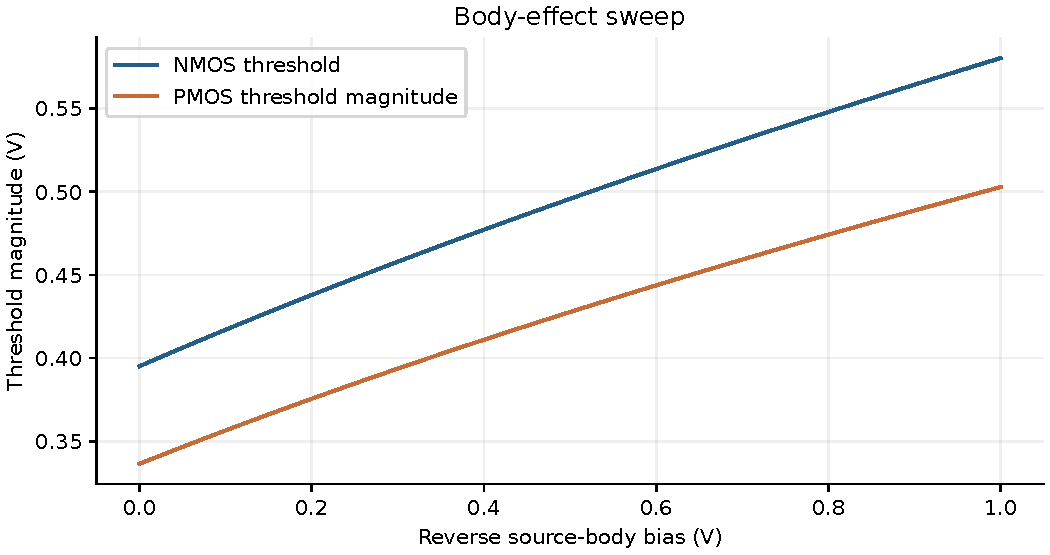
\includegraphics[width=.82\linewidth]{figures/body_threshold.pdf}
\caption{VTH 直接輸出顯示反偏增大時，兩種元件的臨界電壓幅度都增加。}
\end{figure}
\section{討論}
N 增加使迴圈延遲增加，頻率降低。基準反推的每級平均延遲，N=3/5/7 約為 82.94/86.14/86.28 ps；N=3 的波形與每級動態工作點不同，因此不應假設三種級數有完全相同的 $t_p$。

反向 body 偏壓提高臨界電壓、降低可用過驅電壓，使頻率下降。本次順序為基準、只改 PMOS、只改 NMOS、兩者皆改；此順序與講義範例相符，但 PMOS 與 NMOS 單邊偏壓的相對差距是模型及尺寸相依的，不能只憑載子遷移率推論所有製程都相同。

波形保留模型產生的小幅過衝與欠衝，沒有截成理想 0/1 V。這些暫態數值不代表已完成可靠度與接面電流檢查。直接 VTH 掃描也包含偏壓改變造成的其他模型效應，不把它宣稱為純粹長通道公式的參數萃取。

\section{可重現檔案}
本實驗上傳下列 netlist；模型設定以註解標記保留，模型檔與其路徑均不隨報告上傳。執行前須在本機補入合法可用的模型設定。
\begin{itemize}
\item \texttt{01\_ring\_oscillators.sp}
\item \texttt{02\_body\_threshold.sp}
\end{itemize}
每一個變體的完整量測值位於本 lab 的 \texttt{results}，並附代表性波形 CSV、分析結果與規格對照清單。波形 CSV 最多保留 2501 個均勻取樣點；直接量測未降採樣。完整原始 listing 留在本機。

